\documentclass[tikz,border=10pt]{standalone}

% Required packages
\usepackage{tikz}
\usetikzlibrary{
    positioning,
    shapes.geometric,
    arrows.meta,
    fit,
    backgrounds,
    calc
}

% Color definitions
\definecolor{powerblue}{RGB}{74,144,226}
\definecolor{controlorange}{RGB}{230,126,34}
\definecolor{hvred}{RGB}{231,76,60}
\definecolor{outputpurple}{RGB}{155,89,182}
\definecolor{stagebackground}{RGB}{245,245,245}

% Custom block style
\tikzset{
    % Basic block style
    block/.style={
        rectangle,
        draw,
        rounded corners=3pt,
        minimum height=1.2cm,
        minimum width=2cm,
        text centered,
        font=\small\bfseries,
        line width=1pt
    },
    % Power block (blue)
    power block/.style={block, draw, thick, fill=blue!10, minimum width=2.7cm, minimum height=1.3cm, inner sep=5pt, rounded corners=3pt},
    % Control block (green)
    control block/.style={block, draw, thick, fill=green!10, minimum width=2.7cm, minimum height=1.3cm, inner sep=5pt, rounded corners=3pt},
    % High voltage block (red)
    hv block/.style={block, draw, thick, fill=red!10, minimum width=2.7cm, minimum height=1.3cm, inner sep=5pt, rounded corners=3pt},
    % Output block (orange)
    output block/.style={block, draw, thick, fill=orange!10, minimum width=2.7cm, minimum height=1.3cm, inner sep=5pt, rounded corners=3pt},
    % Connection arrows
    arrow/.style={
        -Stealth,
        line width=1pt,
        draw=black
    },
    % Connection labels
    arrow label/.style={
        font=\small\itshape,
        midway,
        above
    },
    % Secondary (discreet) additions: thin grey lines and small labels
    aux/.style={-Stealth, line width=0.6pt, draw=black!55},
    aux label/.style={font=\scriptsize\itshape, text=black!65},
    % Stage encapsulation boxes
    stage box/.style={
        draw=gray!60,
        fill=stagebackground,
        rounded corners=5pt,
        line width=0.8pt,
        inner xsep=8pt,
        inner ysep=10pt
    },
    % Stage title
    stage title/.style={
        font=\small\bfseries,
        anchor=north
    }
}

\begin{document}
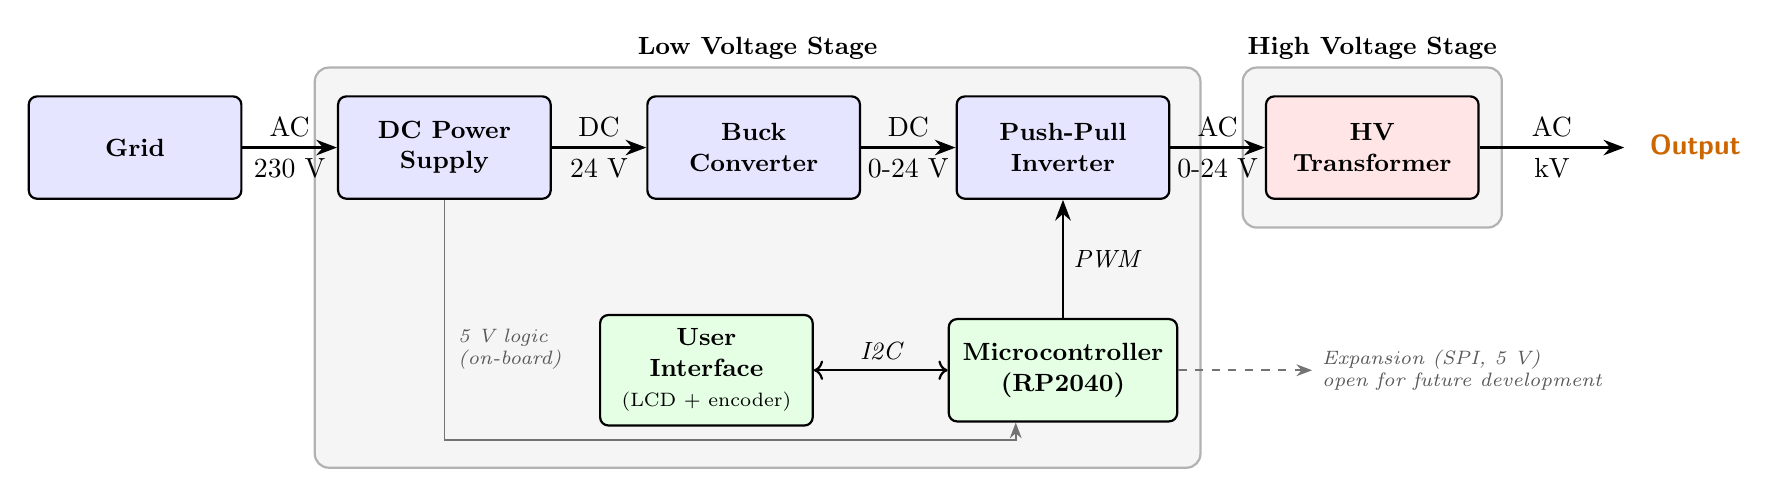
\begin{tikzpicture}[
    node distance=0.8cm and 1.2cm,
    every node/.style={align=center}
]

% ============================================
% BLOCK DEFINITIONS
% Syntax: \node[style] (name) at/position {content};
% ============================================

% --- All Stages Aligned Horizontally ---
\node[power block] (grid) {Grid};
\node[power block, right=of grid] (dcpower) {DC Power\\Supply};
\node[power block, right=of dcpower] (buck) {Buck\\Converter};
\node[power block, right=of buck] (inverter) {Push-Pull\\Inverter};
\node[hv block, right=of inverter] (transformer) {HV\\Transformer};


% --- Control Block ---
\node[control block, below=1.5cm of inverter] (mcu) {Microcontroller\\(RP2040)};
% --- User Interface Block ---
\node[control block, left=1.7cm of mcu] (ui) {User\\Interface\\{\scriptsize\normalfont (LCD + encoder)}};

% ============================================
% CONNECTIONS
% Syntax: \draw[arrow] (from) -- (to) node[arrow label] {label};
% ============================================

% Horizontal connections (All stages)
\draw[arrow] (grid) -- (dcpower) node[above, midway] {AC} node[below, midway] {230 V};
\draw[arrow] (dcpower) -- (buck) node[above, midway] {DC} node[below, midway] {24 V};
\draw[arrow] (buck) -- (inverter) node[above, midway] {DC} node[below, midway] {0-24 V};
\draw[arrow] (inverter) -- (transformer) node[above, midway] {AC} node[below, midway] {0-24 V};
% Output arrow
\draw[arrow] (transformer) -- ++(3.2,0) node[above, midway] {AC} node[below, midway] {kV};
% Output decoration
\node[font=\bfseries\sffamily, anchor=west, align=left] at ($(transformer)+(3.4,0)$) {\textcolor{orange!80!black}{Output}};

% Control signal
\draw[arrow] (mcu.north) -- (inverter.south) node[arrow label, right] {PWM};
% User Interface double arrow
\draw[arrow, <->, thick] (ui) -- (mcu) node[arrow label, above, midway] {I2C};

% Logic supply: 24 V -> on-board 5 V regulator -> MCU
\draw[aux] (dcpower.south) -- ++(0,-3.05) coordinate (lsa) -| ([xshift=-6mm]mcu.south);
\node[aux label, anchor=west, align=left] at ($(dcpower.south)+(0.05,-1.9)$) {5 V logic\\(on-board)};
% Extension ports (left unwired)
\draw[aux, dashed] (mcu.east) -- ++(1.7,0) coordinate (ext)
    node[aux label, right, align=left] {Expansion (SPI, 5 V)\\open for future development};

% ============================================
% STAGE ENCAPSULATION
% Syntax: \begin{scope}[on background layer]
%           \node[stage box, fit=(nodes)] (name) {};
%           \node[stage title] at (name.north) {Title};
%         \end{scope}
% ============================================

\begin{scope}[on background layer]
    % Low Voltage Stage box
    \node[stage box, fit=(dcpower)(buck)(inverter)(mcu)(ui)(lsa)] (lvstage) {};
    \node[stage title] at ($(lvstage.north)+(0,0.5)$) {Low Voltage Stage};

    % High Voltage Stage box
    \node[stage box, fit=(transformer)] (hvstage) {};
    \node[stage title] at ($(hvstage.north)+(0,0.5)$) {High Voltage Stage};
\end{scope}

\end{tikzpicture}
\end{document}
